% !TeX root = ../../tesis.tex

% =============================================================================
\subsubsection{Proyectos cartográficos y plantillas institucionales}
\label{subsubsec:tg-proyectos}
% =============================================================================

La Figura~\ref{fig:tg-arbol} muestra la estructura de directorios completa de
\textbf{Transport-gis}. El repositorio se articula en cinco carpetas de primer
nivel con responsabilidades bien delimitadas: \texttt{analysis/} centraliza los
\textit{scripts} de procesamiento y los cuadernos de exploración;
\texttt{data/processed/} almacena las diez capas \textit{GeoPackage} versionadas
en Git~\textsc{lfs}; \texttt{maps/} agrupa los proyectos QGIS~(\texttt{.qgz}),
las plantillas visuales~(\texttt{.qpt}) con las paletas institucionales de la
\textsc{unam} y el directorio de exportaciones; \texttt{pipeline/} contiene el
orquestador del proceso; y \texttt{setup/} distribuye los activos tipográficos
para garantizar la reproducibilidad visual en distintos sistemas operativos. Los
mapas terminados se exportan en \texttt{.pdf} (alta resolución para la tesis) y
\texttt{.png} (presentaciones del coloquio), cerrando el ciclo descrito en la
Figura~\ref{fig:tg-pipeline}.

\begin{figure}[htbp]
\centering
% Árbol: Estructura de directorios de Transport-gis-zmvm-mjg
% Usado en: 4-Capas-Codigo/4-3-Visualizacion.tex  (fig:tg-arbol)
% Requiere: \usepackage{forest} — declarado en Latex/Comands.tex
\begin{forest}
  for tree = {
    font   = \footnotesize\ttfamily,
    grow'  = 0,
    child anchor  = west,
    parent anchor = east,
    anchor = west,
    draw   = gray!45,
    fill   = gray!7,
    rounded corners = 2pt,
    inner xsep = 6pt,
    inner ysep = 3pt,
    l sep  = 20pt,
    s sep  = 5pt,
    edge path = {
      \noexpand\path [draw=gray!50, thin, rounded corners=2pt]
        (!u.parent anchor) -- +(8pt,0) |- (.child anchor)
        \forestoption{edge label};
    },
  }
  [Transport-gis-zmvm-mjg/, fill=unamAzul!12, draw=unamAzul!70,
                             font=\small\bfseries\ttfamily
    [analysis/
      [notebooks/]
      [scripts/
        [apimetro\_client.py,
          draw=none, fill=none, font=\footnotesize\ttfamily\color{unamAzul}]
        [vft\_runner.py,
          draw=none, fill=none, font=\footnotesize\ttfamily\color{unamAzul}]
      ]
    ]
    [data/processed/
      [{\textit{10 capas .gpkg} \textnormal{(Git~LFS)}},
        draw=none, fill=none, font=\footnotesize\itshape\ttfamily]
    ]
    [maps/, fill=unamOro!8, draw=unamOro!60
      [exports/
        [{\textit{*.pdf · *.png}},
          draw=none, fill=none, font=\footnotesize\itshape\ttfamily]
      ]
      [fonts/]
      [projects/
        [\textit{*.qgz},
          draw=none, fill=none, font=\footnotesize\itshape\ttfamily]
      ]
      [templates/
        [{\textit{*.qpt} \textnormal{(paletas UNAM)}},
          draw=none, fill=none, font=\footnotesize\itshape\ttfamily]
      ]
    ]
    [pipeline/
      [run\_pipeline.py,
        draw=none, fill=none, font=\footnotesize\ttfamily\color{unamAzul}]
    ]
    [setup/
      [install\_fonts.sh,
        draw=none, fill=none, font=\footnotesize\ttfamily\color{unamAzul}]
      [install\_fonts.bat,
        draw=none, fill=none, font=\footnotesize\ttfamily\color{unamAzul}]
    ]
  ]
\end{forest}

\caption[Estructura de directorios de Transport-gis-zmvm-mjg]%
{Árbol de directorios del repositorio \textbf{Transport-gis-zmvm-mjg}. Las
carpetas \texttt{maps/} (oro) y la raíz (azul UNAM)
son los nodos centrales de la producción cartográfica. Los archivos en azul son
\textit{scripts} ejecutables;
  los de fondo plano son activos generados o de datos.}
\label{fig:tg-arbol}
\end{figure}

La Figura~\ref{fig:mapa-red-esquematica} presenta el resultado de este proceso
aplicado a la red de transporte completa de la \zmvm{}: un mapa de síntesis que
integra los doce sistemas reconocidos por el modelo, proyectados en el espacio
metropolitano real. Este mapa constituye la representación cartográfica de
referencia del estudio y es el punto de partida para la interpretación de los
indicadores presentados en el Capítulo~\ref{ch:resultados-vft}. Las versiones de
alta resolución a página completa de todos los mapas producidos por
\textbf{Transport-gis} se encuentran en el Anexo~
\ref{anx:cartografia-presentacion}.

\begin{figure}[htbp]
  \centering
  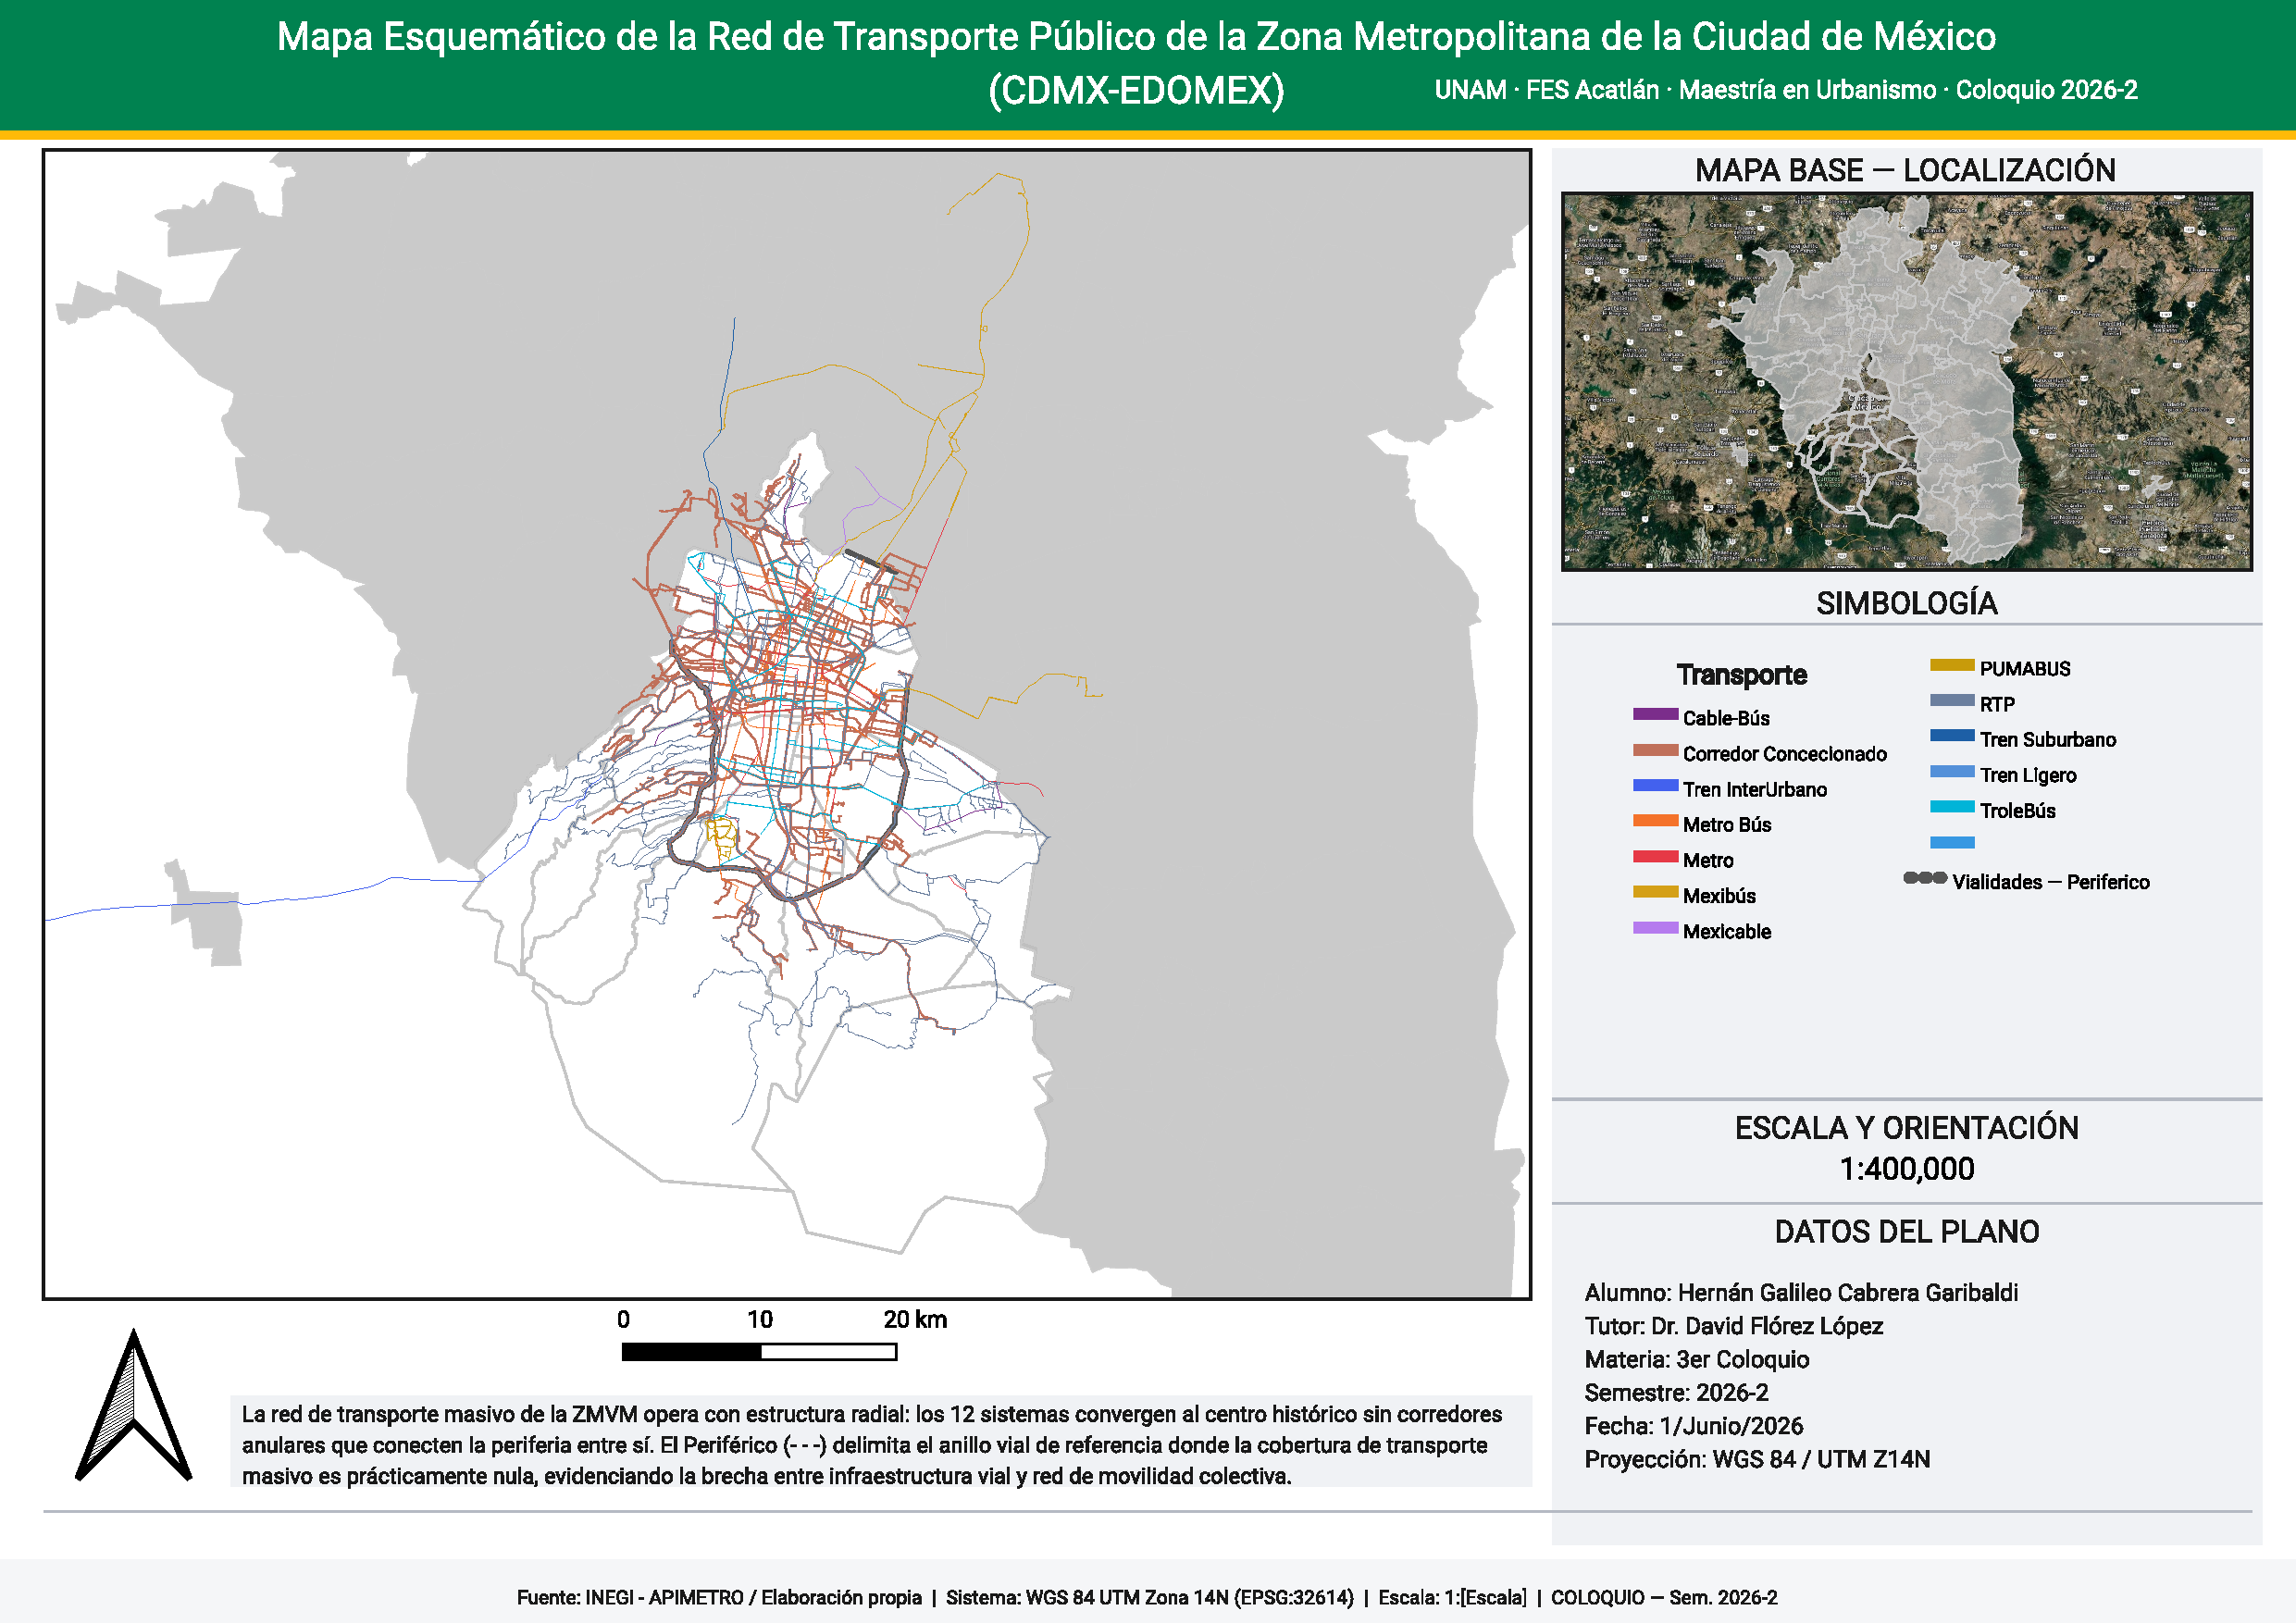
\includegraphics[width=\textwidth]{Figures/Mapas/Mapa_Red_Esquematica}
  \caption[Red multimodal de transporte de la ZMVM]{Red esquemática multimodal de la \zmvm{} generada por \textbf{Transport-gis-zmvm-mjg}.
Incluye los doce sistemas de transporte reconocidos por el modelo, proyectados
en EPSG:32614 (UTM zona~14N) sobre los límites político-administrativos
de la \cdmx{} y el Estado de México.
\fuentefigura{Elaboración propia con QGIS~3.x, plantillas institucionales \textsc{unam};
    datos: \textsc{gtfs} \textsc{semovi} 2024 e \textsc{inegi} 2023.}}
  \label{fig:mapa-red-esquematica}
\end{figure}
